\documentclass{beamer}
\usetheme[
  block=fill, 
  background=dark, 
  titleformat=smallcaps,
  progressbar=frametitle,
  numbering=none,
]{metropolis}
\usepackage{url}
\usepackage{underscore}
\usepackage{xcolor}
\definecolor{dark}{HTML}{23373b}
\definecolor{bright}{HTML}{EB811B}
\definecolor{white}{HTML}{FFFFFF}

\usetikzlibrary{decorations.pathreplacing}

% Tikz
\usepackage{tikz}
\usetikzlibrary{fit,backgrounds, arrows, shapes}
\tikzset{
    example/.style = {
      rounded corners,
      fill = bright,
      outer sep = 2pt,
      inner sep = 1pt,
    },
    task/.style = {
      rounded corners,
      fill=dark,
      text=white,
      text width=2cm,
      align=center
    },
    formula/.style = {
	  rounded corners,
      text=white,
      text width=6cm,
      align=center,
      text centered,
    },
    --/.style = {
      ->,
      dashed, line width = 6pt,
      thick,
      >=stealth
    },
    -->/.style = {
      ->,
      thick,
      -stealth
    },
}
% Beamer
\title{WLP-based Testing}
\subtitle{Progress Report}
\author{Orestis Melkonian}
\institute{Universiteit Utrecht}

% Box macro
\newcommand{\ex}[2]{
  \vfill
  \begin{alertblock}{#1}
    #2
  \end{alertblock}
}

\begin{document}  
	\maketitle
	
	\begin{frame}{Overview}
    \begin{itemize}
      \item{Parsing}
      \item{Calculating paths}
      \item{Renaming}
      \item{Calculating WLP}
      \item{Replacing Conditionals}
      \item{Normalizing}
      \item{SMT-solving}
    \end{itemize}
	\end{frame}
  
	\begin{frame}{Parsing}
	Transforms given GCL file to an internal AST.
	
	\ex{Example}{	 
	    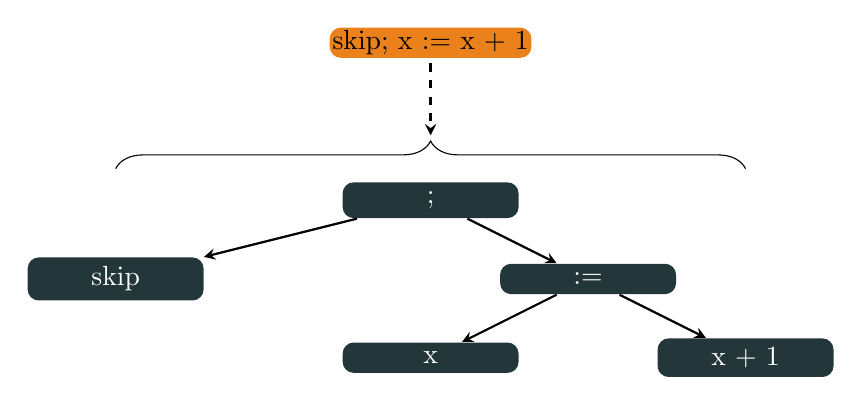
\begin{tikzpicture}
		    \node[example] (EXAMPLE) at (1, 3) {skip; x := x + 1};	  
		    \node          (JOIN) at (1, 1.7) {};
	  
	        \node[task] (SEQ) at (1, 1) {;};
	        \node[task] (SKIP) at (-3, 0) {skip};
	        \node[task] (LHS) at (1, -1) {x};
  	        \node[task] (ASG) at (3, 0) {:=};
 	        \node[task] (RHS) at (5, -1) {x + 1};

		    \draw[--] (EXAMPLE) -- (JOIN);
	 
	 	    \draw[-->] (SEQ) -- (SKIP);
	 	    \draw[-->] (SEQ) -- (ASG);
	 	    \draw[-->] (ASG) -- (LHS);
	 	    \draw[-->] (ASG) -- (RHS);
	 	    \draw [decorate,decoration={brace,amplitude=10pt}] (-3, 1.4) to (5, 1.4);
       \end{tikzpicture} 
	}
	\end{frame}
	
	\begin{frame}{Paths}
	Calculate all possible program paths up to some length. Branching statements are:
	\begin{itemize}
		\item{If-then-else}

		\tikzstyle{hackennode}=[draw,circle,fill=white,inner sep=0,minimum size=4pt]
		\tikzstyle{hackenline}=[line width=3pt]
		\ex{Example}{
\[
\begin{tikzpicture}[baseline=-0.65ex,scale=0.5]
    \draw[draw=none] (-0.5,-1) -- (1,-1);
    \node[hackennode] (middle) at ( 0,   0) {};
    \node[hackennode] (left)   at (-0.5,-1) {};
    \node[hackennode] (right)  at ( 0.5,-1) {};
    \node[hackennode] (top)    at ( 0,   1) {};
    \draw[hackenline,blue] (left) -- (middle) -- (right);
    \draw[hackenline,red] (middle) -- (top);
\end{tikzpicture}
=
\{
\begin{tikzpicture}[baseline=-0.65ex,scale=0.5]
    \draw[draw=none] (-0.5,-1) -- (1,-1);
    \node[hackennode] (middle) at ( 0,   0) {};
	\node[hackennode] (left)   at (-0.5,-1) {};
    \node[hackennode] (top)    at ( 0,   1) {};

    \draw[hackenline,blue] (middle) -- (left);
    \draw[hackenline,red] (middle) -- (top);
\end{tikzpicture}
\tikz[baseline=-0.65ex,scale=0.5] \node[inner sep=0] at (0,-1) {,\,};
\begin{tikzpicture}[baseline=-0.65ex,scale=0.5]
	\draw[draw=none] (-0.5,-1) -- (1,-1);
    \node[hackennode] (middle) at ( 0,   0) {};
    \node[hackennode] (right)  at ( 0.5,-1) {};
    
    \node[hackennode] (top)    at ( 0,   1) {};

    \draw[hackenline,blue] (middle) -- (right);
    \draw[hackenline,red] (middle) -- (top);
\end{tikzpicture}
\}
\]
	}
		
	\item{While}
	\ex{Example}{
\[
\begin{tikzpicture}[baseline=-0.65ex,scale=0.5]
    \draw[draw=none] (-0.5,-1) -- (1,-1);
    \node[hackennode] (bottom)   at (0,-1) {};
    \node[hackennode] (top)    at ( 0,   1) {};
    \draw[hackenline,blue] (top) -- (bottom);
    \node[hackennode] (middle) at ( 0,   0) {};
    \draw[hackenline,red] (middle) -- (top);
\end{tikzpicture}
=
\{
\begin{tikzpicture}[baseline=-0.65ex,scale=0.5]
    \draw[draw=none] (-0.5,-1) -- (1,-1);
	\node[hackennode] (mid)   at ( 0,  0) {};
	\node[hackennode] (bottom)   at ( 0,  -1) {};
    \draw[hackenline,red] (mid) -- (bottom);
\end{tikzpicture}
\tikz[baseline=-0.65ex,scale=0.5] \node[inner sep=0] at (0,-1) {,\,};
\begin{tikzpicture}[baseline=-0.65ex,scale=0.5]
    \draw[draw=none] (-0.5,-1) -- (1,-1);
	\node[hackennode] (top)    at ( 0,   1) {};	
	\node[hackennode] (mid)   at ( 0,  0) {};
	\node[hackennode] (bottom)   at ( 0,  -1) {};
    \draw[hackenline,red] (top) -- (mid);
    \draw[hackenline,blue] (mid) -- (bottom);
\end{tikzpicture}
\tikz[baseline=-0.65ex,scale=0.5] \node[inner sep=0] at (0,-1) {,\,};
\begin{tikzpicture}[baseline=-0.65ex,scale=0.5]
    \draw[draw=none] (-0.5,-1) -- (1,-1);
	\node[hackennode] (top)    at ( 0,   1) {};	
	\node[hackennode] (mid)   at ( 0,  .3) {};
	\node[hackennode] (midd)   at ( 0,  -.3) {};
	\node[hackennode] (bottom)   at ( 0,  -1) {};
    \draw[hackenline,red] (top) -- (mid);
    \draw[hackenline,blue] (mid) -- (midd);
    \draw[hackenline,blue] (midd) -- (bottom);
\end{tikzpicture}
\tikz[baseline=-0.65ex,scale=0.5] \node[inner sep=0] at (0,-1) {\ldots\,};
\}
\]
	}	
	
	\end{itemize}
	\end{frame}  	

	\begin{frame}{Renaming}
	Rename all locally-scoped variables in:
	\begin{itemize}
		\item{Var statements}
		\ex{Example}{\center{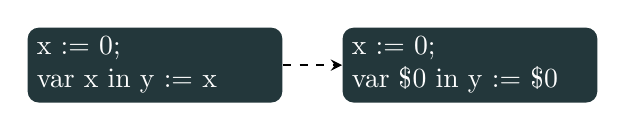
\begin{tikzpicture}
		    \node[task, text width=3cm] (A) at (-2, 0) {
		    	\begin{minipage}{2\textwidth}  	
					x := 0; \newline var x in y := x		    	
		    	\end{minipage}
		    };	  
	        \node[task, text width=3cm] (B) at (2, 0) {
	        	\begin{minipage}{2\textwidth}
	        		x := 0; \newline var \alert{\$0} in y := \alert{\$0}
		        \end{minipage}
	        };
		    \draw[--] (A) -- (B);
        \end{tikzpicture}}}		
		
		\item{Forall expressions}
		\ex{Example}{\center{
\begin{tikzpicture}
		    \node[task, text width=3cm] (A) at (-2, 0) {
		    	\begin{minipage}{2\textwidth}  	
		    		x = 0 $\Rightarrow$ \newline $\forall$ x :: y = x
		    	\end{minipage}
		    };	  
	        \node[task, text width=3cm] (B) at (2, 0) {
	        	\begin{minipage}{2\textwidth}
	        		x = 0 $\Rightarrow$ \newline $\forall$ \alert{\$0} :: y = \alert{\$0}
		        \end{minipage}
	        };
		    \draw[--] (A) -- (B);
        \end{tikzpicture}}}	
		
		
	\end{itemize}
	\end{frame}  	  	
	
	\begin{frame}{WLP}
	For each path, calculate its weakest precondition.
	
	\ex{Issue}{Handle array assignments.}
	\ex{Solution}{Use \alert{repby} and, when indexed, convert to conditional expressions.}

	\end{frame}  	
	
	\begin{frame}{Conditional replacement}
	Array assignments introduce conditional expressions to the final logical formula.
	\ex{Example}{\[
		wlp \,\, (a[1] := 10) \,\, (a[5] = 1) \Longrightarrow (1 = 5 \rightarrow 10 \, | \, a[5]) = 1
	\]}
	
	Replace these with primitive logical formulas.
	\ex{Example}{\[
	(g \rightarrow lhs\,|\,rhs) = E \,\,\equiv\,\, (g \Rightarrow lhs = E) \land (\neg g \Rightarrow rhs = E)
	\]}
	
	
	\end{frame}
	
	\begin{frame}{Normalizing}
	Normalize the form of the result WLP formula to:
	\begin{itemize}
		\item{A list of assumptions}
		\item{The final goal}
	\end{itemize}
	 
	
	\ex{Example}{
		\begin{tikzpicture}
		    \node[formula] (A) at (0, 1)
		    {\[ A_1 \Rightarrow A_2 \Rightarrow ... \Rightarrow A_n \Rightarrow G \]};
	        \node[formula] (B) at (0, -1)
	        {\[ A_1 \land A_2 \land ... \land A_n \Rightarrow G \]};
	 	    \draw[-->] (A) -- (B);
	   \end{tikzpicture}
	}
	\end{frame}

	\begin{frame}{SMT-solving}
	SAT-solve the conjuction of the assumptions:
	
	\begin{itemize}
		\item{\alert{Unsatisfiable} $\rightarrow$ Infeasible path}
		\item{\alert{Satisfiable} with model $[ x \leadsto x' ] \rightarrow$
		\begin{itemize}
			\item{\textcolor{green}{Pass}, if $G[x' / x]$ }
			\item{\textcolor{red}{Fail}, if $\neg G[x' / x]$ }
		\end{itemize}}
	\end{itemize}
	
	\ex{Issue}{Still have to handle arrays, as they appear in the formula.}
	\ex{Solution}{Treat them as uninterpreted symbols.}

	\end{frame}  


\end{document}